\documentclass[12pt,twoside,a4paper]{report}
\usepackage[a4paper,width=150mm,top=25mm,bottom=25mm,bindingoffset=6mm]{geometry}

\usepackage[utf8x]{inputenc}
\usepackage[slovak]{babel}
\usepackage{palatino,verbatim}

% Balicek pre priamu rec - \say
\usepackage{dirtytalk}

% Balicek "alltt" je to iste ako "verbatim" mod, ale navyse podporuje aj formatovacie znacky textu
\usepackage{alltt}

% Obrazky
\usepackage{graphicx}
\graphicspath{ {obr/} }

% Cislovanie obrazkov a tabuliek
\usepackage{chngcntr}
%Cisluj obrazky nezavisle od cisla kapitol/podkapitol
\counterwithout{figure}{subsection}
\counterwithout{table}{subsection}

% Referencovanie kapitol/sekcii/... podľa ich nadpisu
\usepackage{nameref}

% Tabulky s viacriadkovymi bunkami a zlucenymi bunkami
% Tabulky generujem naastrojom "http://www.tablesgenerator.com/"
\usepackage{booktabs}
\usepackage{multirow}
% LaTeX ma problemy s prikazmi cline a cmidrule, ked je babel nastaveny na slovencinu/cestinu, kvoli definicii pomlcky
\usepackage{etoolbox}
\preto\tabular{\shorthandoff{-}}

%Uloz obrazok tam, kde je deklarovany
%\usepackage[subsection]{placeins}

\newcommand\sktxt[1]{\foreignlanguage{slovak}{#1}}

\begin{document}
\pagenumbering{arabic}

\setcounter{chapter}{1}
\chapter*{Distribúcia multicastovej prevádzky}
\paragraph{}
Andrej Šišila, Marián Vachalík

\tableofcontents

\newpage
\section{Topológia}
\paragraph{}
Budeme konfigurovať distribúciu multicastovej prevádzky so smerovacím protokolom IS-IS na topológií, ktorá je znázornená na obrázku \ref{fig:mcast_isis_topo}. IP adresácia je uvedená v tabuľke \ref{tab:ip_adresacia} a dopĺňa grafické znázornenie topológie na obrázku \ref{fig:mcast_isis_topo}.

\begin{figure}[!htb]
\centering
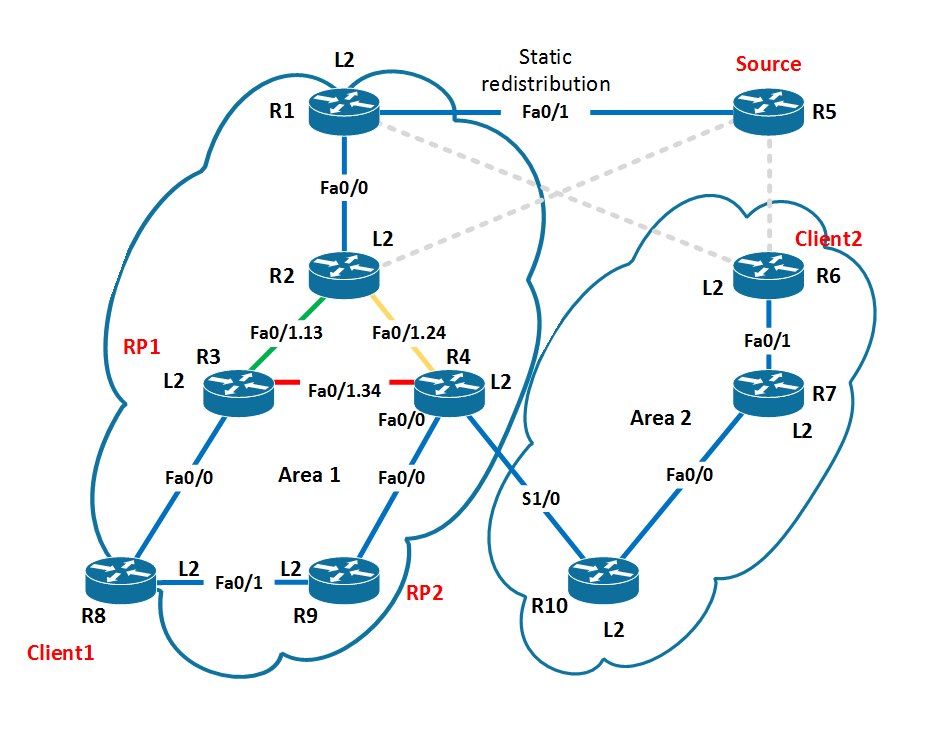
\includegraphics[width=12cm,keepaspectratio]{mcast_isis_topo}
\caption{Topológia IS-IS}
\label{fig:mcast_isis_topo}
\end{figure}



\begin{table}[!htb]
\centering
\caption{IP adresácia}
\label{tab:ip_adresacia}
\begin{tabular}{|c|c|l|l|l|}
\hline
\multicolumn{1}{|c|}{\textbf{Smerovač}}    & \multicolumn{1}{c|}{\textbf{Funkcia}}                        & \multicolumn{1}{c|}{\textbf{Rozhranie}} & \multicolumn{1}{c|}{\textbf{IP adresa}} & \multicolumn{1}{c|}{\textbf{Maska}} \\ \hline
\multirow{3}{*}{R1}  & \multirow{3}{*}{L2}                   & Fa0/0                                   & 10.0.12.1                               & 255.255.255.0                       \\ \cline{3-5} 
                     &                                         & Fa0/1                                   & 10.100.15.1                             & 255.255.255.0                       \\ \cline{3-5} 
                     &                                         & Lo0                                     & 10.255.255.1                            & 255.255.255.255                     \\ \hline
\multirow{3}{*}{R2}  & \multirow{3}{*}{L2}             & Fa0/0                                   & 10.0.12.2                               & 255.255.255.0                       \\ \cline{3-5} 
                     &                                         & Fa0/1                                   & 10.0.234.2                             & 255.255.255.0                       \\ \cline{3-5}
                     &                                         & Lo0                                     & 10.255.255.2                            & 255.255.255.255                     \\ \hline
\multirow{4}{*}{R3}  & \multirow{4}{*}{L1/L2}                    & Fa0/0                                   & 10.1.38.3                               & 255.255.255.0                       \\ \cline{3-5} 
                     &                                         & Fa0/1                                   & 10.0.234.3                              & 255.255.255.0                       \\ \cline{3-5} 
                     &                                         & S1/0                                    & 10.2.39.3                               & 255.255.255.252                     \\ \cline{3-5} 
                     &                                         & Lo0                                     & 10.255.255.3                            & 255.255.255.255                     \\ \hline
\multirow{4}{*}{R4}  & \multirow{4}{*}{L1/L2}                    & Fa0/0                                   & 10.2.49.4                               & 255.255.255.0                       \\ \cline{3-5} 
                     &                                         & Fa0/1                                   & 10.0.234.4                              & 255.255.255.0                       \\ \cline{3-5} 
                     &                                         & S1/0                                    & 10.3.104.4                              & 255.255.255.252                     \\ \cline{3-5} 
                     &                                         & Lo0                                     & 10.255.255.4                            & 255.255.255.255                     \\ \hline
\multirow{2}{*}{R5}  & \multirow{2}{*}{Smerovač iného systému} & Fa0/1                                   & 10.100.15.5                             & 255.255.255.0                       \\ \cline{3-5} 
                     &                                         & Lo0                                     & 10.255.255.5                            & 255.255.255.255                     \\ \hline
\multirow{2}{*}{R6}  & \multirow{2}{*}{L1}             & Fa0/0                                   & 10.4.67.6                               & 255.255.255.0                       \\ \cline{3-5} 
                     &                                         & Lo0                                     & 10.255.255.6                            & 255.255.255.255                     \\ \hline
\multirow{3}{*}{R7}  & \multirow{3}{*}{L1}             & Fa0/1                                   & 10.4.67.7                               & 255.255.255.0                       \\ \cline{3-5} 
                     &                                         & S1/1                                    & 10.4.107.7                              & 255.255.255.0                       \\ \cline{3-5} 
                     &                                         & Lo0                                     & 10.255.255.7                            & 255.255.255.255                     \\ \hline
\multirow{2}{*}{R8}  & \multirow{2}{*}{L1}             & Fa0/0                                   & 10.1.38.8                               & 255.255.255.0                       \\ \cline{3-5} 
                     &                                         & Lo0                                     & 10.255.255.8                            & 255.255.255.255                     \\ \hline
\multirow{3}{*}{R9}  & \multirow{3}{*}{L1}             & Fa0/0                                   & 10.2.49.9                               & 255.255.255.0                       \\ \cline{3-5} 
                     &                                         & S1/0                                    & 10.2.39.9                               & 255.255.255.0                       \\ \cline{3-5} 
                     &                                         & Lo0                                     & 10.255.255.9                            & 255.255.255.255                     \\ \hline
\multirow{3}{*}{R10} & \multirow{3}{*}{L1/L2}                    & S1/0                                    & 10.3.104.10                              & 255.255.255.0                       \\ \cline{3-5} 
                     &                                         & S1/1                                    & 10.4.107.10                              & 255.255.255.0                       \\ \cline{3-5} 
                     &                                         & Lo0                                     & 10.255.255.10                           & 255.255.255.255                     \\ \hline
\end{tabular}
\end{table}


% Novu kapitolu davam na novu stranu, lebo bez toho mi zobrazuje tabulku v dalsej kapitole, kde ale tabulka nepatri.
\newpage


\section{Úlohy}
\subsection{Konfigurácia PIM Dense Mode}
\label{konfiguracia_pim_dense_mode}
\subsubsection{Popis}
Úlohou bolo najprv sa oboznámiť s konfiguráciou PIM Dense Mode. Dohodli sme sa, že budeme používať iba smerovací protokol IS-IS.
Subrozhranie “.13” a VLAN 13 sme premenovali na “.23” a VLAN 23, lebo sieť je medzi smerovačmi R2 a R3 (23), a nie medzi R1 a R3 (13).

\paragraph{}
V rámci tohto zadania sme použili IS–IS (L2 only) s jednou oblasťou a priame point-to-point prepojenia medzi R2, R3, R4. Takisto sme použili R5 ako zdroj multicastovej prevádzky. R6 a R8 sme nakonfigurovali ako multicast klientov.

\paragraph{}
IP adresa multicastovej skupiny bola \say{239.0.0.1}.


\subsubsection{Konfigurácia}
\paragraph{}
Nižšie je uvedená konfigurácia pre klientský smerovač R6. Rozhranie pridáme do IS-IS protokolu príkazom \say{ip router isis}. V nastaveniach procesu ISIS (\say{router isis}) sme definovali Lo0 ako pasívne rozhranie (neposielajú sa Hello pakety), nastavili sme NSAP identifikátor príkazom \say{net}, typ priľahlosti pre R1 sme nastavili ako L2 príkazom \say{is-type level-2}, a nakoniec sme nastavili rozšírenú metriku pre R1 príkazom \say{metric-style wide}. Rozšírená metrika je novšou implementáciou počítania metriky pre IS-IS. Pokiaľ sa rozhodneme použiť takúto metriku, musíme ju nastaviť na všetkých smerovačoch v IS-IS doméne.

\paragraph{}
Následne sme nakonfigurovali PIM Dense Mode. Multicast režim aktivujeme príkazom \say{ip multicast-routing} v globálnom konfiguračnom režime. Potom pre jednotlivé rozhrania povolíme multicastové smerovanie príkazom \say{ip pim dense-mode}. Klientov, t.j. Lo1, pridávame do multicastovej skupiny skupiny príkazom \say{igmp join-group 239.0.0.1} v rámci konfigurácie rozhrania.

\noindent
{\fontfamily{qcr}\selectfont
\begin{small}
\begin{alltt}
!R6
ena
conf t
hostname R6
no ip domain-lookup
username admin privil 15 secret admin
line con 0
  login local
  logging syn
  exec-time 120
line vty 0 15
  privilege level 15
  no login
int f0/1
  ip addr 10.2.67.6 255.255.255.0
  ip router isis
  isis network point-to-point
  no shut
int lo0
  ip addr 10.255.255.6 255.255.255.255
  ip router isis
  no shut
int lo1
  ip add 10.255.255.66 255.255.255.255
  ip router isis
  ip igmp join-group 239.0.0.1
router isis
  net 49.0002.0102.5525.5006.00
  passive-interface lo0
  is-type level-2
  metric-style wide
  exit

!aktivujeme multicast smerovanie
ip multicast-routing
int range f0/1
  ip pim dense-mode
  exit
int lo0
  ip pim dense-mode
  exit
int lo1
  ip pim dense-mode
  exit
\end{alltt}
\end{small}
}

\subsubsection{Overenie}

\noindent
{\fontfamily{qcr}\selectfont
\begin{small}
\begin{alltt}
R5#ping 239.0.0.1

Type escape sequence to abort.
Sending 1, 100-byte ICMP Echos to 239.0.0.1, timeout is 2 seconds:

Reply to request 0 from 10.1.38.8, 68 ms
Reply to request 0 from 10.2.67.6, 132 ms


----------------------------------------------------------------


R8#sh ip pim interface

Address          Interface         Ver/   Nbr    Query  DR     DR
                                   Mode   Count  Intvl  Prior
10.255.255.88    Loopback1         v2/D   0      30     1      10.255.255.88
10.1.38.8        FastEthernet0/0   v2/D   1      30     1      10.1.38.8
10.1.89.8        FastEthernet0/1   v2/D   1      30     1      10.1.89.9
10.255.255.8     Loopback0         v2/D   0      30     1      10.255.255.8

\end{alltt}
\end{small}
}

\paragraph{}
Po vykonaní ping-u na IP adresu multicastovej skupiny nám prišli odpovede z oboch klientských smerovačov: R6 a R8. Výpis príkazu \say{show ip pim interface} zo smerovača R8 dokazuje, že všetky rozhrania sú nastavené v \say{Dense} móde (v stĺpci \say{Ver/Mode} vidíme \textbf{D}, čo indikuje aktívny \say{Dense} mód).













\subsection{Konfigurácia PIM Sparse Mode}
\subsubsection{Popis}
Konfigurujeme \say{Sparse} mód (šetrný mód) s jedným RP bez záložného RP. Úlohu RP plnil smerovač R3 \say{Sparse} mód, narozdiel od \say{Dense} módu, nezahlcuje sieť správami na odpojenie od skupiny (tzv. \say{PRUNE} správy), čím šetrí vyťaženie smerovačou. Namiesto toho posiela multicastový tok iba tým, ktorí si o to požiadajú tzv. \say{JOIN} správou. Na preposielanie týchto správ sa používa zdieľaný strom, ktorého \say{koreňom} je Rendezvous (čítaj \textit{randevú}) Point (ďalej len RP smerovač). RP smerovač pozná všetky zdroje, z ktorých sa šíri  multicastový tok a následne ho preposiela multicastovým klientom.

\subsubsection{Konfigurácia}
\paragraph{}
Nižšie je uvedená konfigurácia R1. IS-IS konfigurácia zostáva totožná s tou v kapitole \ref{konfiguracia_pim_dense_mode}. Multicast režim aktivujeme príkazom \say{ip multicast-routing} v globálnom konfiguračnom režime. Rozhranie pridáme do PIM Sparse Mode procesu príkazom \say{ip pim sparse-mode}. RP nastavíme v globálnom konfiguračnom režime príkazom \say{ip pim rp-addr 10.255.255.3}

\noindent
{\fontfamily{qcr}\selectfont
\begin{small}
\begin{alltt}
!R1
!aktivujeme multicast smerovanie
ip multicast-routing
int range f0/0 - 1
  ip pim sparse-mode
int lo0
  ip pim sparse-mode
  exit
ip pim rp-addr 10.255.255.3
\end{alltt}
\end{small}
}


\subsubsection{Overenie}

\noindent
{\fontfamily{qcr}\selectfont
\begin{small}
\begin{alltt}
R5#ping 239.0.0.1

Type escape sequence to abort.
Sending 1, 100-byte ICMP Echos to 239.0.0.1, timeout is 2 seconds:

Reply to request 0 from 10.1.38.8, 60 ms
Reply to request 0 from 10.2.67.6, 124 ms
\end{alltt}
\end{small}
}

\noindent
{\fontfamily{qcr}\selectfont
\begin{small}
\begin{alltt}

R3#sh ip pim int

Address          Interface            Ver/   Nbr    Query  DR     DR
                                      Mode   Count  Intvl  Prior
10.1.38.3        FastEthernet0/0      v2/S   1      30     1      10.1.38.8
10.1.23.3        FastEthernet0/1.23   v2/S   1      30     1      10.1.23.3
10.1.34.3        FastEthernet0/1.34   v2/S   1      30     1      10.1.34.4
10.255.255.3     Loopback0            v2/S   0      30     1      10.255.255.3
\end{alltt}
\end{small}
}


\paragraph{}
Rovnako ako pri \say{Dense} móde, pri ping-u na IP adresu multicastovej skupiny prichádzali odpovede od klientov 10.1.38.8 (R8) a 10.2.67.6 (R6). Výpis príkazu \say{show ip pim interface} hovorí, že rozhrania na smerovači R3 sú v \say{Sparse} móde (viď písmeno \textbf{S} v stĺpci \say{Ver/Mode}, čo značí aktívny \say{Sparse} mód).










\subsection{Konfigurácia PIM Sparse−Dense Mode a zabezpečenie RP redundancie}
\subsubsection{Popis}
\paragraph{}
V \say{Sparse-Dense} móde môžeme nastaviť záložný RP, ktorý bude vyberaný pomocou BSR. \say{Sparse} mód je používaný na šírenie multicastového toku, \say{Dense} mód na šírenie informácie o prítomnosti RP smerovača.

\subsubsection{Konfigurácia}

\noindent
{\fontfamily{qcr}\selectfont
\begin{small}
\begin{alltt}
!R1
!aktivujeme multicast smerovanie
ip multicast-routing
int range f0/0 - 1
  ip pim sparse-dense-mode
int lo0
  ip pim sparse-dense-mode
  exit
no ip pim rp-addr 10.255.255.3

!R3
!aktivujeme multicast smerovanie
ip multicast-routing
int f0/0
  ip pim sparse-dense-mode
int f0/1.23
  ip pim sparse-dense-mode
int f0/1.34
  ip pim sparse-dense-mode
int lo0
  ip pim sparse-dense-mode
  exit
no ip pim rp-addr 10.255.255.3
ip pim rp-candidate lo0

!R9
!aktivujeme multicast smerovanie
ip multicast-routing
int range f0/0 - 1
  ip pim sparse-dense-mode
  exit
int lo0
  ip pim sparse-dense-mode
no ip pim rp-addr 10.255.255.3
ip pim bsr-candidate lo0
\end{alltt}
\end{small}
}

\subsubsection{Overenie}

\noindent
{\fontfamily{qcr}\selectfont
\begin{small}
\begin{alltt}
R5#ping 239.0.0.1

Type escape sequence to abort.
Sending 1, 100-byte ICMP Echos to 239.0.0.1, timeout is 2 seconds:

Reply to request 0 from 10.1.89.8, 76 ms
Reply to request 0 from 10.2.67.6, 136 ms


---------------------------------------------------------------------------


R4#sh ip pim rp
Group: 239.0.0.1, RP: 10.255.255.3, v2, uptime 00:04:27, expires 00:02:19


---------------------------------------------------------------------------


R4#sh ip pim int

Address          Interface            Ver/   Nbr    Query  DR     DR
                                      Mode   Count  Intvl  Prior
10.1.49.4        FastEthernet0/0      v2/SD  1      30     1      10.1.49.9
10.1.24.4        FastEthernet0/1.24   v2/SD  1      30     1      10.1.24.4
10.1.34.4        FastEthernet0/1.34   v2/SD  1      30     1      10.1.34.4
10.1.104.4       Serial1/0            v2/SD  1      30     1      0.0.0.0
10.255.255.4     Loopback0            v2/SD  0      30     1      10.255.255.4


---------------------------------------------------------------------------


R9#sh ip igmp groups
IGMP Connected Group Membership
Group Address  Interface        Uptime    Expires   Last Reporter   Group
                                                                    Accounted
224.0.1.39     FastEthernet0/0  00:11:57  00:01:57  10.1.49.4
224.0.1.40     FastEthernet0/0  01:03:32  00:02:59  10.1.49.4


---------------------------------------------------------------------------

\end{alltt}
\end{small}
}


\noindent
{\fontfamily{qcr}\selectfont
\begin{small}
\begin{alltt}
Power Tools

R6#mstat 10.100.15.5 224.0.1.40
Type escape sequence to abort.
Mtrace from 10.100.15.5 to 10.2.67.6 via group 224.0.1.40
From source (?) to destination (?)
Waiting to accumulate statistics......
Results after 10 seconds:

  Source        Response Dest   Packet Statistics For     Only For Traffic
10.100.15.5     10.2.67.6       All Multicast Traffic     From 10.100.15.5
     |       __/  rtt 87   ms   Lost/Sent = Pct  Rate     To 224.0.1.40
     v      /     hop 87   ms   ---------------------     --------------------
10.100.15.1
10.1.12.1       ?
     |     ^      ttl   0
     v     |      hop -8   s     0/0 = --%      0 pps    0/0 = --%  0 pps
10.1.12.2
10.1.24.2       ?
     |     ^      ttl   1
     v     |      hop 2576 ms    0/0 = --%      0 pps    0/0 = --%  0 pps
10.1.24.4
10.1.104.4      ?
     |     ^      ttl   2
     v     |      hop 15   s     0/0 = --%      0 pps    0/0 = --%  0 pps
10.1.104.10
10.2.107.10     ?
     |     ^      ttl   3
     v     |      hop -8   s     0/0 = --%      0 pps    0/0 = --%  0 pps
10.2.107.7
10.2.67.7       ?
     |     ^      ttl   4
     v     |      hop -1   s     0/0 = --%      0 pps    0/0 = --%  0 pps
10.2.67.6       ?
     |      \__   ttl   5
     v         \  hop 0    ms        0         0 pps           0    0 pps
10.2.67.6       10.2.67.6
  Receiver      Query Source

\end{alltt}
\end{small}
}

\paragraph{}
Rovnako ako pri \say{Dense} móde, pri ping-u na IP adresu multicastovej skupiny prichádzali odpovede od klientov 10.1.38.8 (R8) a 10.2.67.6 (R6). Výpis príkazu \say{show ip pim interface} hovorí, že rozhrania na smerovači R3 sú v \say{Sparse-Dense} móde (viď písmeno \textbf{SD} v stĺpci \say{Ver/Mode}, čo značí aktívny \say{Sparse-Dense} mód). Z výpisu príkazu \say{show ip pim rp} vidíme IP adresu multicastovej skupiny pre klientov a IP adresu RP smerovača, čo je adresa loopback0 rozhrania pre R3.  Vo výpise príkazu \say{show ip igmp groups} vidíme, že smerovač R1 patrí do multicastovej skupiny \say{224.0.1.40}, čo je AutoRP Discovery. AutoRP je Cisco implemenácia hľadania záložného RP smerovača pomocou RP-Mapper smerovača. Do tejto skupiny patria predvolene všetky Cisco smerovače.

\paragraph{}
Po ping-u na multicastovú adresu prišli odpovede od oboch klientských smerovačov: R6 a R8. Výpis príkazu \say{sh ip pim rp} ukazuje, že RP smerovač je R3, o čom hovorí adresa loopback0 rozhrania. Výpis príkazu \say{show ip pim interface} hovorí, že všetky rozhrania na smerovači R4 sú v \say{Sparse-Dense} móde. Príkaz \say{show ip igmp groups} ukazuje, že smerovač R9 patrí do multicastových skupín: 224.0.1.40 (RP Discovery) a 224.0.1.39 (RP Announce). Tým, že patrí aj do skupiny \say{RP Announce} oznamuje ostatným smerovačom, že môže byť kandidátom na RP, čo je dôkaz, že záložný RP je v pohotovosti. Príkaz \say{show ip pim autorp} zo smerovača R4 hovorí, že \say{AutoRP} protokol na vyhľadanie záložného RP smerovača je aktívny, čo je dôkaz, že smerovač R4 funguje správne ako \say{RP Mapper}. Nakoniec príkaz \say{mstat} vykreslil zdieľaný strom od zdroja (R5) ku klientovi (R6) cez multicastovú skupinu 224.0.1.40.







\subsection{Zmerať konvergenciu v prípade výpadku}
\subsubsection{Popis}
Vypli sme linku \say{Fa0/1.23} medzi R2 a R3 zmenou IP adresy na chybnú (z 10.1.23.3 na 10.2.23.3).

\subsubsection{Konfigurácia}
\paragraph{}

\noindent
{\fontfamily{qcr}\selectfont
\begin{small}
\begin{alltt}
R3(config)#int f0/1 
R3(config-if)#int f0/1.23     
R3(config-subif)#ip address 10.2.23.3 255.255.255.248
*Mar  2 23:53:39.844: %PIM-5-DRCHG: DR change from neighbor 10.1.23.3 to\\10.2.23.3 on interface FastEthernet0/1.23

\end{alltt}
\end{small}
}


Kontrola konvergencie zo smerovača R5:

\noindent
{\fontfamily{qcr}\selectfont
\begin{small}
\begin{alltt}

R5#ping        
Protocol [ip]:             
Target IP address: 10.255.255.8
Repeat count [5]: 10000000    
Datagram size [100]:
Timeout in seconds [2]: 1           
Extended commands [n]:
Sweep range of sizes [n]:
Type escape sequence to abort.
Sending 10000000, 100-byte ICMP Echos to 10.255.255.8, timeout is 1 seconds:
!!!!!!!!!!!!!!!!!!!!!!!!!!!!!!!!!!!!!!!!!!!!!!!!!!!!!!!!!!!!!!!!!!!!!!
!!!!!!!!!!!!!!!..............!!!!!!!!!!!!!!!!!!!!!!!!!!!!!!!!!!!!!!!!!
!!!!!!!!!!!!!!.
Success rate is 98 percent (770/785), round-trip min/avg/max = 56/81/112 ms

\end{alltt}
\end{small}
}

\paragraph{}
Nakoniec sme merali konvergenciu pri celkovom výpadku RP (R3).

\noindent
{\fontfamily{qcr}\selectfont
\begin{small}
\begin{alltt}
*Mar  5 23:05:28.230: %PIM-5-NBRCHG: neighbor 10.1.23.3 UP on interface \\FastEthernet0/1.23 
*Mar  5 23:05:28.282: %PIM-5-DRCHG: DR change from neighbor 0.0.0.0 to \\10.1.23.3 on interface FastEthernet0/1.23
\end{alltt}
\end{small}
}

\noindent
{\fontfamily{qcr}\selectfont
\begin{small}
\begin{alltt}

R1#show ip pim rp mapping
PIM Group-to-RP Mappings

Group(s) 224.0.0.0/4
  RP 10.255.255.3 (?), v2
    Info source: 10.255.255.9 (?), via bootstrap, priority 0, holdtime 150
         Uptime: 4d20h, expires: 00:02:13

\end{alltt}
\end{small}
}

\paragraph{}
Kontrola ukázala, že zmena RP smerovača na R9 po výpadku R3 sa uskutočnila za cca 50ms, avšak smerovaciemu protokolu IS-IS trvalo približne 14 sekúnd, kým aj klientský smerovač R8 získal konektivitu so zvyškom siete.

\subsection{Otázky}
\paragraph{}
1. Prvých 25 bitov multicastovej MAC-adresy?\\
A. 01-00-5e +\\
B. 01-00-01\\
C. 09-00-01\\
D. 08-09-07\\

\paragraph{}
2. Ako môžeme vybrať RP?\\
A. Static RP +\\
B. BSR +\\
C. Smart RP\\
D. Auto RP +\\

\paragraph{}
3. Čo je to RP?\\
A. Začiatok multicast stromu\\
B. Koniec multicast stromu\\
C. Začiatok zdieľaného stromu +\\
D. Miesto stretnutia pre zdroj a prijímač +\\

\paragraph{}
4. Koľko bitov multicast IP adresy sa mapuje na multicast MAC adresu?\\
A. 27\\
B. 23 +\\
C. 25\\
D. 26\\

\paragraph{}
5. V akom móde sa vytvára zdieľaný strom?\\
A. Dense mód\\
B. Sparse mód +\\
C. Auto RP mód\\
D. Zieľaný strom sa nevytvára\\

\end{document}